\chapter{Grundlagen}\label{s:grundlagen}

\section{Stumpfk\"orperaerodynamik (TG)}

%	Stumpfkörper
%	D-Stumpfkörper
%	Strömungsfeld
%	Ablösung
%	Totwasser
%	Wirbelschichten
%	Nachlauf
%	Praktische Bedeutung
%	Ggf. Vergleich schlanke Körper

Im folgenden Kapitel wird der Begriff der Stumpfk"orper und deren Unterschiede zu den schlanken K"orpern eingef"uhrt. Eine klare Abgrenzung von schlanken K"orpern zu Stumpfk"orpern bereitet Schwierigkeiten, da der "Ubergang oftmals flie\ss{}end ist. Jedoch unterscheidet sich die Aerodynamik markant, weswegen im folgenden Kapitel im Besonderen auf das Str"omungsbild und die Charakteristiken des Nachlaufs eingegangen werden sollen.

\subsection{Geometrische Einordnung}
\label{sec:Geometrie}
Ein stumpfer K"orper in einer Anstr"omung differenziert sich geometrisch von einem schlanken insofern, dass er eine signifikante Dicke quer zur Anstr"omung aufweist, welche in vergleichbarer Gr"o\ss{}enordnung wie die Abmessungen parallel zur Anstr"omung liegt. Als Ma\ss{} kann das Dickenverh"altnis $\sigma$ als Kehrwert des Schlankheitsgrades $\lambda$ herangezogen werden, welches das Verh"altnis der Dicke $d$ zur L"ange $l$ wiedergibt:

\begin{align}
\sigma = \frac{1}{\lambda} = \frac{d}{l}
\end{align}

Wie in \abb{fig:HuchoDV} zu sehen ist, ver"andert sich das Str"omungsbild ma\ss{}geblich mit steigendem Dickenverh"altnis $\sigma$, wobei der "Ubergang von schlanken K"orpern ($\sigma = 0,13$) zu stumpfen K"orpern ($\sigma = 0,5$) flie\ss{}end ist.

\begin{figure}[h]
	\centering
	\begin{subfigure}[c]{0.45\textwidth}		
		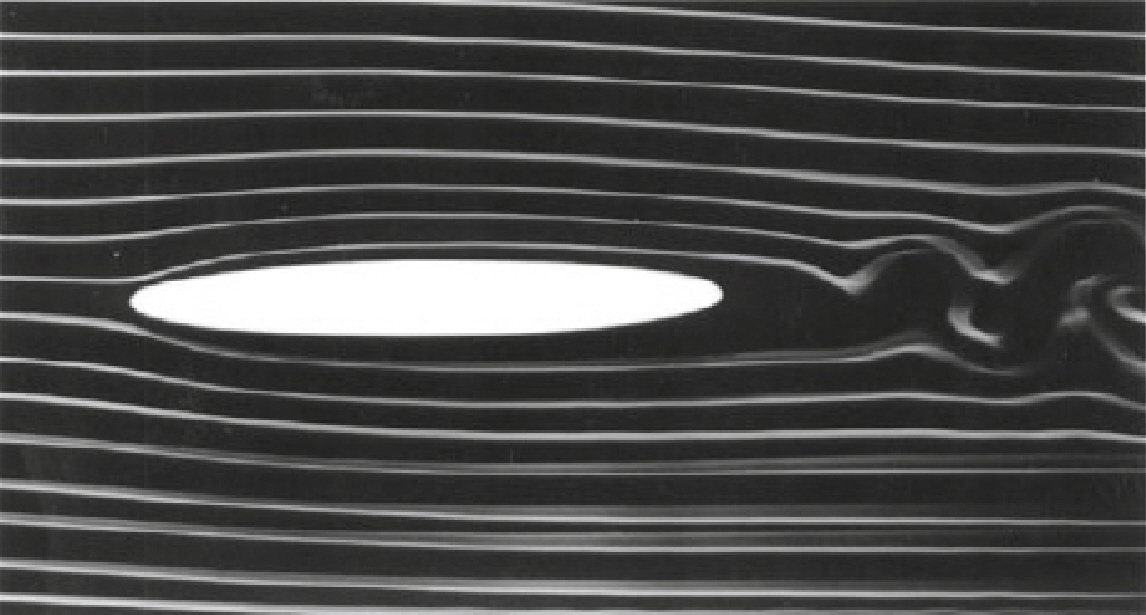
\includegraphics[width=1\textwidth]{HuchoDV013.jpg}
		\subcaption{$\sigma = 0,13$}
	\end{subfigure}
	\begin{subfigure}[c]{0.45\textwidth}
		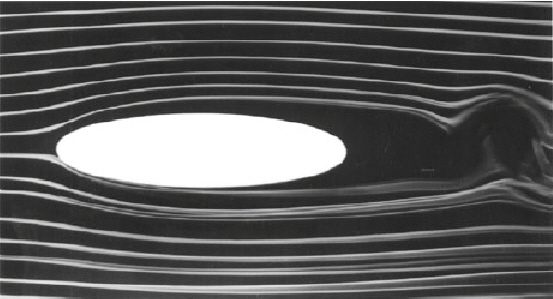
\includegraphics[width=1\textwidth]{HuchoDV026.jpg}
		\subcaption{$\sigma = 0,26$}
	\end{subfigure}
	\begin{subfigure}[c]{0.45\textwidth}
		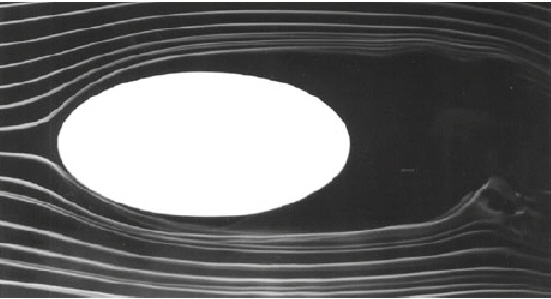
\includegraphics[width=1\textwidth]{HuchoDV05.jpg}
		\subcaption{$\sigma = 0,5$}
	\end{subfigure}
	\caption{elliptische Zylinder unterschiedlicher Dickenverh"altnisse im Rauchkanal \cite{Hucho.2011}}
	\label{fig:HuchoDV}
\end{figure}

Obwohl das Dickenverh"altnis in allgemeiner N"aherung ein gutes Ma\ss{} f"ur die Einordnung eines Stumpfk"orpers ist, zeigt sich in der Praxis, dass es nicht als notwendiges Kriterium herangezogen werden kann. So treten vergleichbare Effekte der Stumpfk"orperaerodynamik ebenfalls bei einem diskontinuierlichen Verlauf der K"orpergeometrie auf. Dies ist beispielsweise bei der ausgepr"agten Hinterkanten eines Fahrzeughecks der Fall. Der Verlauf der K"orpergeometrie muss also ebenfalls als geometrische Charakterisierung eines stumpfen K"orpers herangezogen werden.


\subsection{Str"omungsbild}
\label{sec:Stromungsbild}
Bei der Umstr"omung eines K"orpers kommt es aufgrund der Haftbedingung an dessen Kontur zur Ausbildung einer Grenzschicht. W"ahrend die Str"omungsgeschwindigkeit an der K"orperoberfl"ache Null betr"agt, passt sie sich im Grenzschichtbereich an die Anstr"omgeschwindigkeit an. Ein Teil der kinetischen Energie der Grenzschichtstr"omung wird durch Reibung an der Wand dissipiert.
Die Geometrie eines stumpfen K"orpers, wie in \abb{fig:HuchoDV} dargestellt, f"uhrt bei Umstr"omung gem"a\ss{} Bernoulli zu einer Absenkung des statischen Drucks $p$ bis zur dicksten Stelle. Hinter dieser steigt der statische Druck $p$ wieder an, wobei die durch Reibung verringerte kinetische Energie nicht mehr ausreicht, um gegen diesen anzustr"omen. Ist die kinetische Energie vollends in Druck umgewandelt, kommt es zur R"uckstr"omung, wobei die Grenzschicht abl"ost \cite{Hucho.2011}.\\
Sofern eine diskontinuierlichen Stelle in der K"orpergeometrie vorhanden ist, kann die Str"omung dieser ebenfalls nicht weiter folgen. Man spricht in diesem Fall von einem Abriss der Str"omung, welcher in der Praxis an Hinterkanten zu finden ist.\\
Das Abl"osen oder Abrei\ss{}en hat die Ausbildung eines Totwassers zur Folge, in dessen Gebiet sich das Fluid bedingt durch Z"ahigkeitseffekte verwirbelt und Wirbelschichten ausbildet. Dies f"uhrt zu einer Druckabsenkung hinter dem stumpfen K"orper, sodass durch den h"oheren Staupunktdruck an der Vorderseite ein Druckgradient zu verzeichnen ist. Ein Druckwiderstand ist die Folge, welcher in Str"omungsrichtung des Fluides wirkt. Wie man in \abb{fig:HuchoStumpf} sehen kann, ist das Totwasser ein Charakteristikum des Str"omungsbildes stumpfer K"orper. Im Vergleich dazu ist dieses Gebiet beim Str"omungsbild schlanker K"orper, wie in \abb{fig:HuchoSchlank} zu sehen, nicht vorhanden. Die Kontur schlanker K"orper erm"oglicht ein nahezu st"orungsfreies Abstr"omen. Lediglich die Reibungseffekte innerhalb der Grenzschichtstr"omung sorgen hier f"ur einen Reibungswiderstand. Schluss folglich wird der Gesamtwiderstand bei stumpfen K"orpern vom Druckwiderstand, der bei schlanken K"orpern jedoch vom Reibungswiderstand dominiert.

\begin{figure}[h]
	\centering
	\includegraphics[width=0.4\textwidth]{HuchoschlankerKorper.jpg}
	\caption{Stromlinienbild eines schlanken K"orpers im Rauchkanal \cite{Hucho.2011}}
	\label{fig:HuchoSchlank}
\end{figure}

\begin{figure}[h]
	\centering
	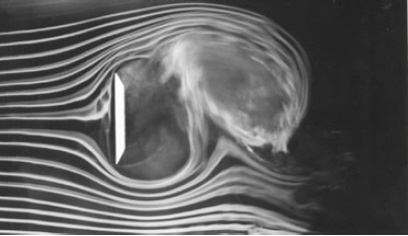
\includegraphics[width=0.4\textwidth]{HuchoStumpferKorper.jpg}
	\caption{Stromlinienbild eines stumpfen K"orpers im Rauchkanal \cite{Hucho.2011}}
	\label{fig:HuchoStumpf}
\end{figure}

Hieraus wird die Notwendigkeit ersichtlich, eine Druckerh"ohung in diesem Totwasser vorzunehmen, um den Druckgadienten und damit den Druckwiderstand zu verringern. F"ur das bessere Verst"andnis soll im nachfolgenden das Totwasser weiter spezifiziert werden.

\subsection{Totwasser}
\label{sec:Totwasser}
Das Totwasser hat im Wesentlichen drei kennzeichnende Eigenschaften. Zum Einen tritt im Innern eine zirkulierende Str"omung auf, welche stark turbulent ist. Des Weiteren bilden sich periodisch alternierende Wirbel und zudem herrscht ein Unterdruck, der r"aumlich nicht konstant ist. Die Ursache dieser Eigenschaften soll im Folgenden beschrieben werden. \\
Wie bereits oben erw"ahnt wurde, bilden sich innerhalb des Totwassers Wirbelschichten aus. Die ehemalige Grenzschichtstr"omung, welche abl"ost, wird zur Scherschichtstr"omung und durchmischt sich turbulent mit dem ruhenden Fluid im Windschatten des K"orpers. Dabei wird das Totwasser selbst besonders durch die Form der Scherschicht gepr"agt, wie in Abbildung \ref{fig:Scherschichten} zu sehen ist. Bei der zweiseitigen Abl"osung, wie das in der dem Experiment zu Grunde liegenden Konfiguration der Fall ist, beeinflussen sich die Scherschichten gegenseitig. Dies ist besonders deutlich aus \abb{fig:HuchoStumpf} ersichtlich.\\
Aufgrund der R"uckstr"omung im Totwasser, bilden sich hinter dem Stumpfk"orper zwei gegenl"aufige Wirbel aus. Diese sind in \abb{fig:Nachlauf}b ersichtlich. Die Wirbel, wachsen durch den eingebrachten Impuls der Scherschichten. Dabei verlagert sich deren Zentrum stark, bis sie die Scherschicht auf der gegen"uberliegenden Seite mit entgegengesetzter Rotation einsaugen. Dadurch l"osen sich die Wirbel abwechselnd ab, sodass sich unter Idealbedingungen eine K\'arm\'ansche Wirbelstra\ss{}e ausbildet. Diese ist in \abb{fig:Wirbelstrasse} zu sehen. \\

\begin{figure}[h]
	\centering
	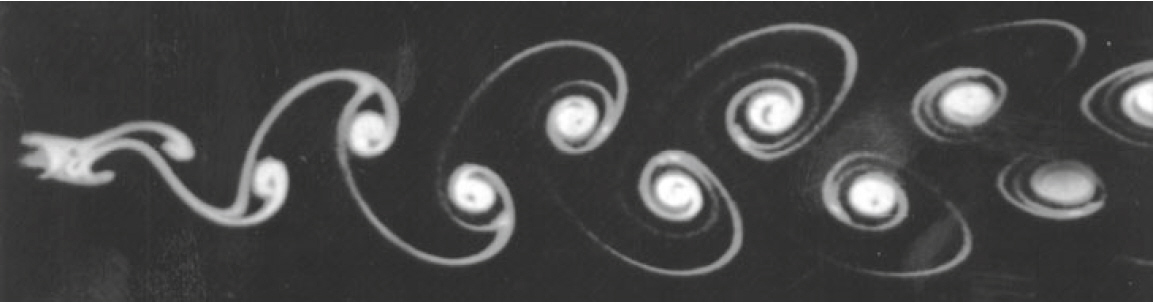
\includegraphics[width=0.7\textwidth]{Wirbelstrasse.jpg}
	\caption{K\'arm\'ansche Wirbelstra\ss{}e \cite{Hucho.2011}}
	\label{fig:Wirbelstrasse}
\end{figure}


Wegen dieser gegenseitigen Beeinflussung ist die Str"omung innerhalb des Totwassers mit zweiseitiger Abl"osung instation"ar und periodisch. Dies f"uhrt zu Druckschwankungen und der bereits beschriebenen Oszillation der Abl"osungen. Um diese Schwingung zu beschreiben, wurde die dimensionslose Strouhal-Zahl $Str$ eingef"uhrt \cite{Leder.1992}. Gem"a\ss{} Gleichung \ref{eq:Str} ist sie dabei abh"angig von der Abl"osefrequenz der Wirbel $f$, der Dicke des Stumpfk"orpers $D$ sowie der Anstr"omgeschwindigkeit $U_{\infty}$. F"ur D-Stumpfk"orper nimmt die Strouhalzahl den Wert $Str = 0,26$ an \cite{Pastoor.2008}.

\begin{align}
	{Str}=\frac{f \cdot D}{U_{\infty}}	
	\label{eq:Str}
\end{align}


W"ahrend sich bei der einseitigen Scherschicht ein langes Totwassergebiet mit hohem Druck ausbildet, ist das Totwasser bei der zweiseitigen Abl"osung k"urzer und der Druck niedriger. Die rotationssymmetrische Abl"osung f"uhrt zu einem Aufrollen der Scherschicht, was daf"ur sorgt, dass der Druck h"oher als im einseitigen Totwasser ist. Die umliegende Str"omung verh"alt sich gegen"uber dem Totwasser in allen drei F"allen so, als w"are es  ein fester K"orper. Es bildet sich eine Trennstromlinie an dessen Rand \cite{Hucho.2011}. 

\begin{figure}[h]
	\centering
	\begin{subfigure}[c]{0.35\textwidth}
		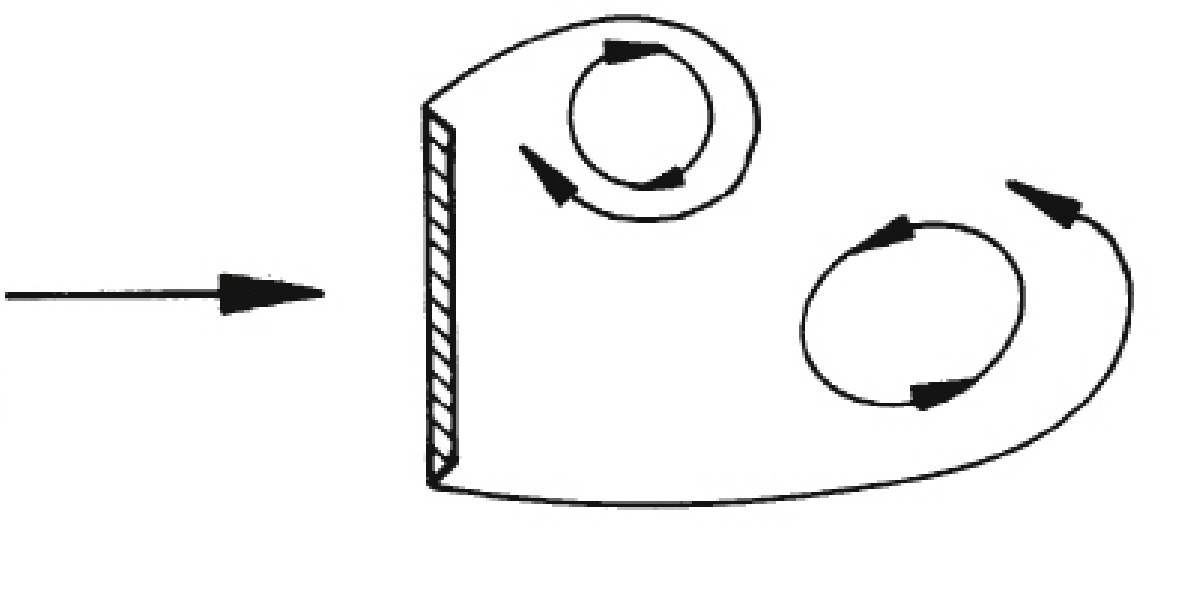
\includegraphics[width=1\textwidth]{ScherSzweiseitig.jpg}
		\subcaption{zweiseitig}
		\label{fig:Scherungzweiseitig}
	\end{subfigure}
	\begin{subfigure}[c]{0.35\textwidth}		
		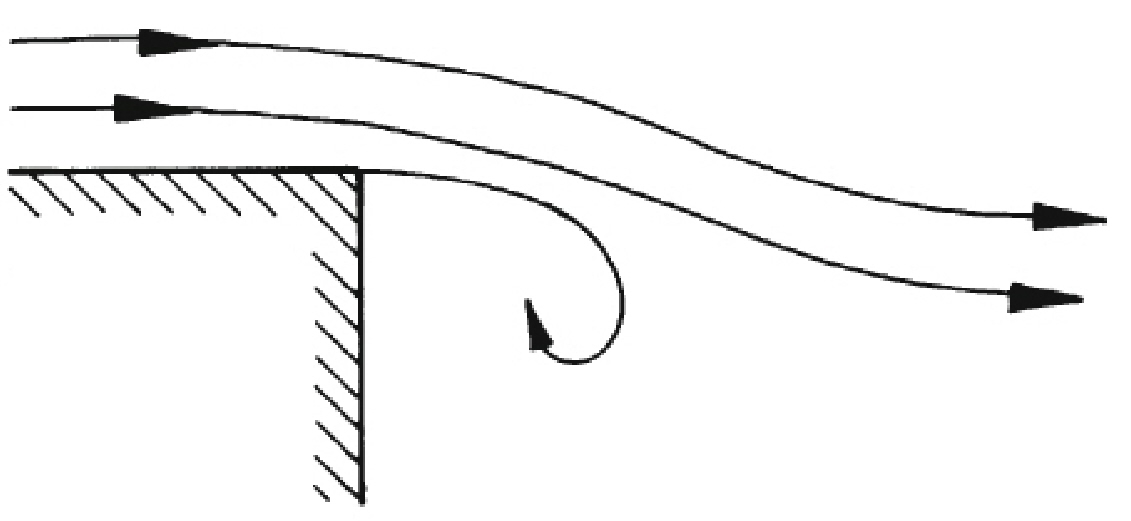
\includegraphics[width=1\textwidth]{ScherSeinseitig.jpg}
		\subcaption{einseitig}
		\label{fig:Scherungeinseitig}
	\end{subfigure}
	\begin{subfigure}[c]{0.35\textwidth}
		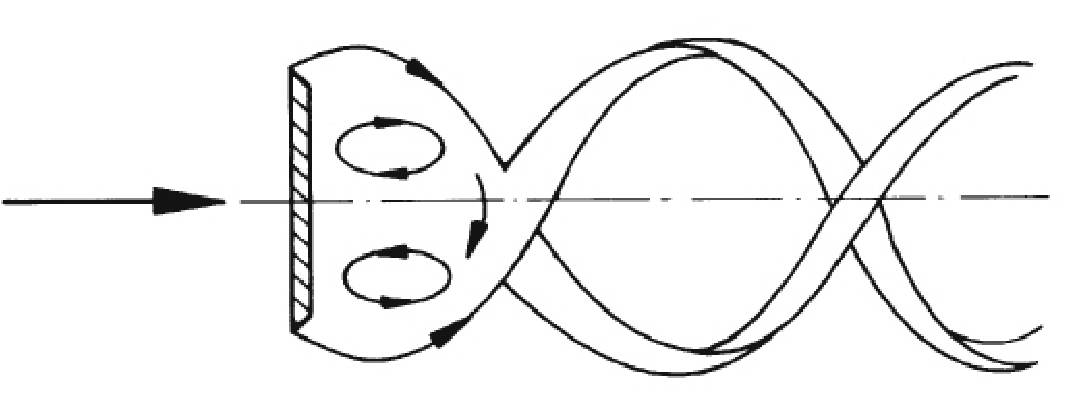
\includegraphics[width=1\textwidth]{ScherSrot.jpg}
		\subcaption{rotationssymmetrisch}
		\label{fig:Scherungrotatorisch}
	\end{subfigure}
	\caption{ Scherschichten \cite{Hucho.2011}}
	\label{fig:Scherschichten}
\end{figure}
 

 \begin{figure}[h]
	\centering
	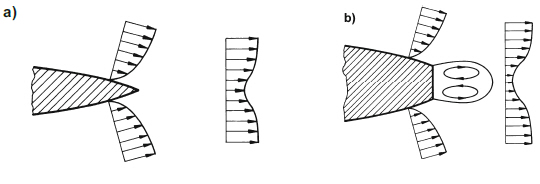
\includegraphics[width=0.9\textwidth]{Nachlauf.jpg}
	\caption{Nachlauf eines a) schlanken K"orpers und eines b) stumpfen K"orpers \cite{Hucho.2011}}
	\label{fig:Nachlauf}
\end{figure}

Da das Totwasser wie ein fester K"orper an der Trennstromlinie umstr"omt wird, kann dort ebenfalls der statische Druck $p$ bei einer entsprechenden Kontur ansteigen. Ist der Druckanstieg zu stark, l"ost das umstr"omende Medium nach dem selben Prinzip wie in Abschnitt \ref{sec:Stromungsbild} ab. Dies bezeichnet man als Abl"osung zweiter Art \cite{Leder.1992}. Dieser Vorgang erfolgt kaskadenartig, sodass sich immer kleinere Wirbel bilden. Bei diesem Vorgang wird Energie  in W"arme dissipiert, bis die Wirbel sich g"anzlich aufl"osen und sich erneut ein laminares Str"omungsprofil ausbildet. Im Nachlauf des Stumpfk"orpers, welcher sich an das Totwasser anschlie\ss{}t, ergibt sich dabei eine Delle im Geschwindigkeitsfeld. Das ist in Abbildung \abb{fig:Nachlauf} zu sehen. Aus dem Nachlauf lassen sich deshalb Informationen "uber den Widerstand des K"orpers ziehen, was in Kapitel \ref{s:widerstandsbestimmung} weiter thematisiert wird.

\subsection{Einfluss der Vorderkante} 
\label{sec:Vorderkante}
Wie sp"ater noch in Abschnitt \ref{sec:Modell} weiter erl"autert wird, handelt es sich bei dem Versuchsmodell um einen D-Stumpfk"orper. Vereinfacht ist dies ein Quader mit stumpfer Vorderkante.\\ 
An einer scharfen Vorderkante l"ost die Str"omung ab und bildet eine laminare Abl"oseblase, was nichts anderem als einem lokal begrenztem Wirbel entspricht. Ein "ahnlicher Vorgang tritt bei der Anstr"omung von Profilen bei kleinen Reynoldszahlen auf, wie es schematisch in \abb{fig:LamBlase} zu sehen ist. Dabei wandelt sich von Punkt A zu Punkt T die laminare in eine turbulente Scherschicht um. Die Turbulenz sorgt f"ur einen Energietransport quer zur Anstr"omung, was dazu f"uhrt, dass die Abl"oseblase von oben geschlossen wird und die Str"omung stromabw"arts am Punkt W wieder anlegt \cite{Siegman.2015}. Der Ort des Wiederanlegens wurde von Ota \& Itasaka \cite{Ota.1976} bei einer ebenen Platte auf $4,5 \cdot \frac{x}{d}$ bestimmt. Da dieser Ort jedoch stark fluktuiert und gro\ss{}e Schwankungen in der Geschwindigkeitsverteilung hervorruft, wird ein Gleichgewicht innerhalb der Grenzschicht erst nach einer Laufl"ange von $\frac{x}{d} = 15$ erreicht.
  
\begin{figure}[h]
	\centering
	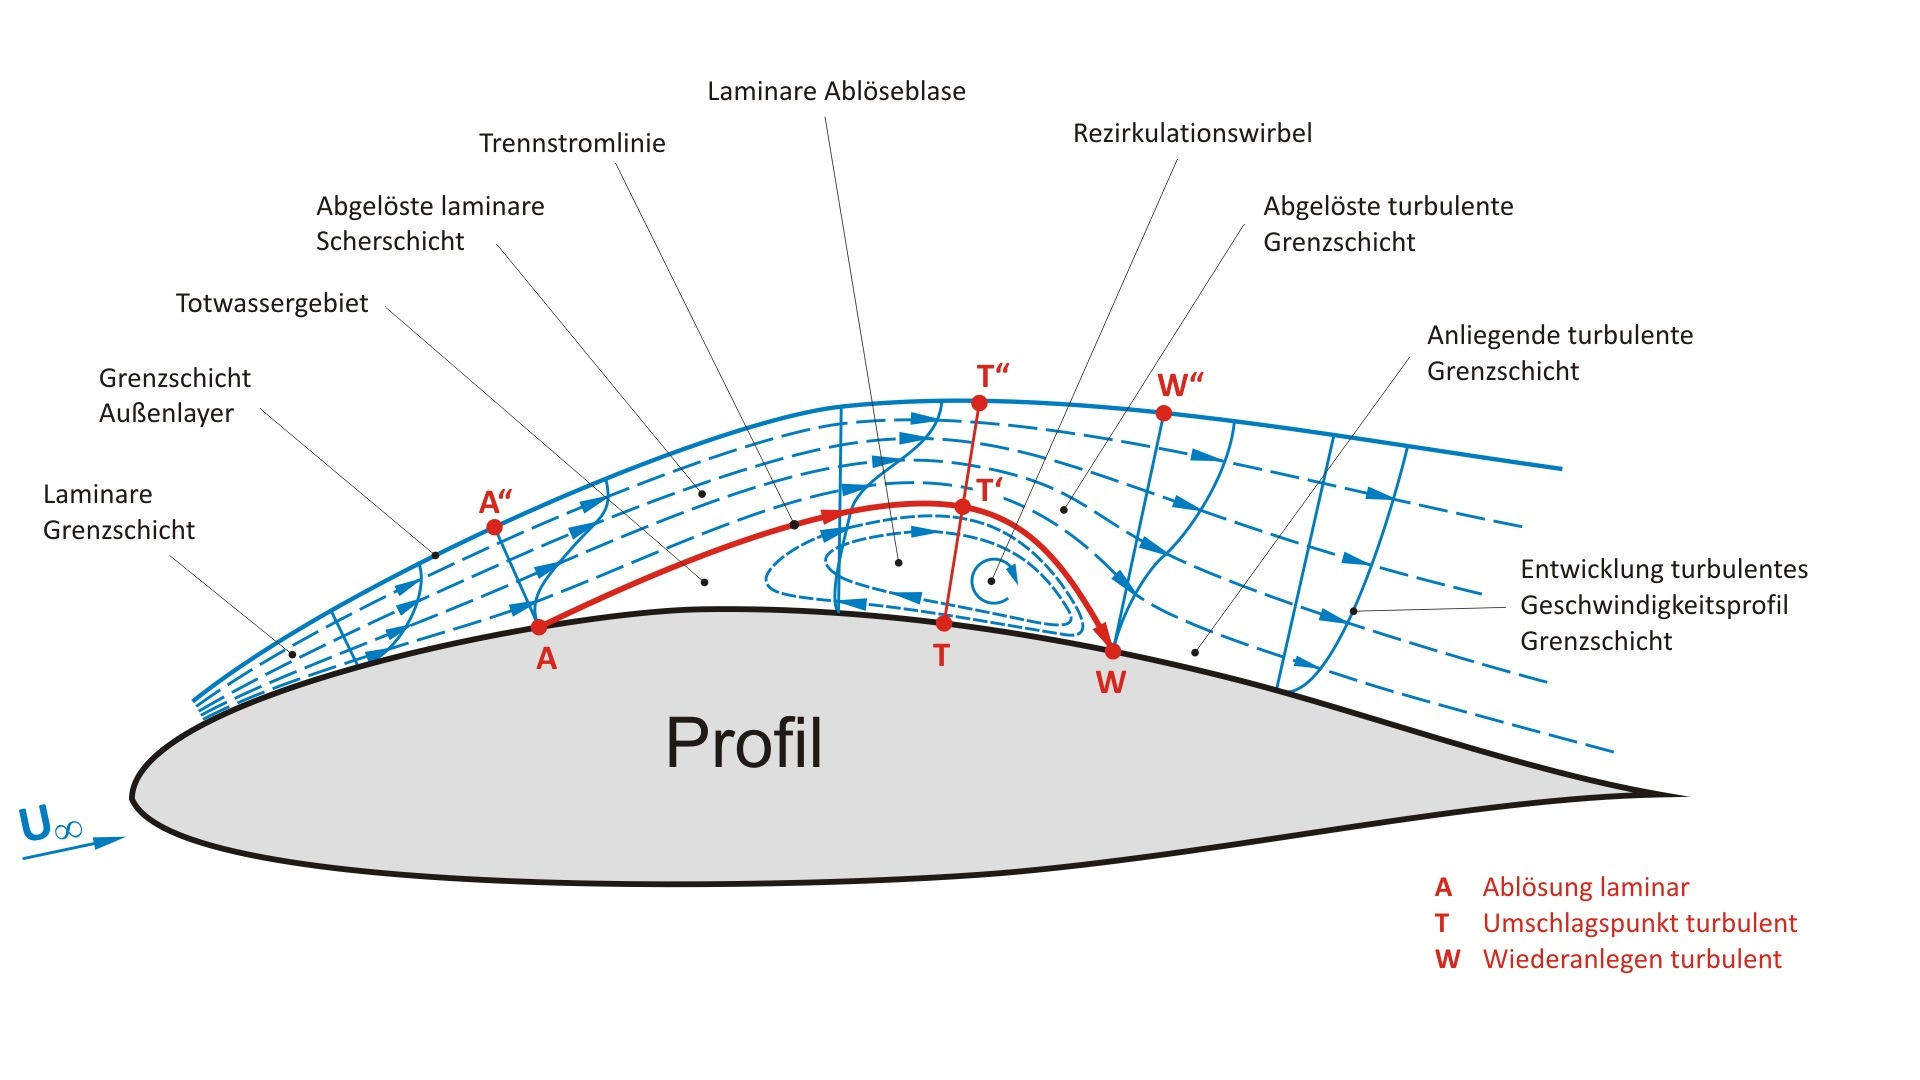
\includegraphics[width=1\textwidth]{LaminareAbloeseblase.jpg}
	\caption{Schema einer laminaren Abl"oseblase \cite{Siegman.2015}}
	\label{fig:LamBlase}
\end{figure}

Aus diesem Grund ist ersichtlich, weshalb die Verwendung eines D-Stumpfk"orpers, der gegen"uber einem Quader abgerundete  Vorderkante hat, sinnvoll ist. Aus der Grafik \abb{fig:Vorderkante} ist die starke Reduktion des Widerstandbeiwertes $C_w$ bei steigendem $\frac{r}{d}$-Verh"altnis f"ur verschiedene Vorderkantengeometrien ersichtlich. Wie der Gegen"uberstellung \abb{fig:Vorderkante} ebenfalls zu entnehmen ist, sinkt der $C_w$-Wert ab der "Uberschreitung eines bestimmten $\frac{r}{d}$-Verh"altnis nicht weiter. Der durch st"arkere Abrundung nach vorne wandernde Ort des Wiederanlegens f"allt ab der "Uberschreitung dieses Verh"altnisses mit dem Ort der Abl"osung zusammen, sodass der Widerstand bei weiterer Abrundung nicht weiter sinkt \cite{Hucho.2011}. 
Um in der Messung lediglich den Einfluss des Totwassers zu ermitteln, ist es deswegen notwendig, das Auftreten von laminaren Abl"oseblasen bestm"oglichst zu reduzieren. Dazu wird an der Vorderkante ein Zackenband angebracht, dessen Auswirkung in Abschnitt \ref{sec:Modell} weiter erl"autert wird.

\begin{figure}[h]
	\centering	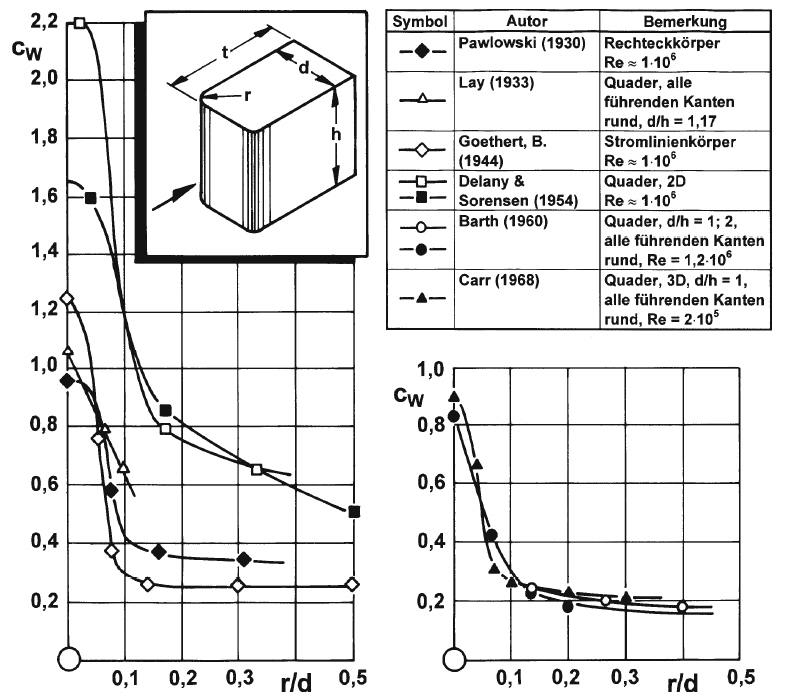
\includegraphics[width=0.6\textwidth]{Vorderkante.jpg}
	\caption{$C_w$-Wert in Abh"angigkeit vom Kantenradius bei verschiedenen 2D-Profilen. Zusammenstellung nach Hucho\cite{Hucho.1972}}
	\label{fig:Vorderkante}
\end{figure}



%\begin{figure}[h]
%	\centering	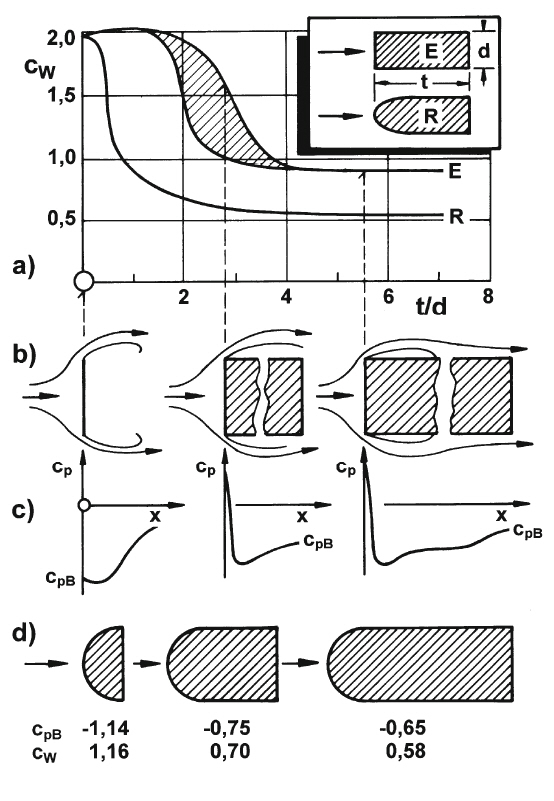
\includegraphics[width=0.6\textwidth]{Vorderkante2.jpg}
%	\caption{Umstr"omung scharfkantiger und stumpfer Vorderkanten in Abh"angigkeit der Profiltiefe t. Zusammenstellung nach Hucho\cite{Hucho.1972}\\ a) $C_w$-Wert \\ b) schematische Str"omungsform \\ c) schematischer Druckverlauf d) Basisdruck und Widerstand}
%	\label{fig:Vorderkante}
%\end{figure}


%\subsection{Praktische Bedeutung der Stumpfk"orper}
%tbd



\section{Coand\^{a}-Effekt (TG)}
%	Umströmung gekrümmter Flächen
%	Haftbedingung
%	Typische Strömungsbilder
%	technische Anwendung 

Da in der dem Experiment zu Grunde liegenden Konfiguration "uber Coand\^{a}-Fl"achen ausblasen wird, um eine bessere Umlenkung in das Totwassergebiet zu erzielen, soll der zu Nutze gemachte Effekt im  nachfolgenden Unterkapitel n"aher beschrieben werden.

Der Coand\^{a}-Effekt tritt auf, wenn ein Strahl entlang einer konvexen K"orperkontur str"omt. Anders als die bisher betrachtete Str"omung, kann die sogenannte Coand\^{a}-Str"omung des Strahles der Kontur einer konvexen Rundung folgen ohne abzul"osen, wie dies in \abb{fig:coanda} deutlich wird. Im Vergleich dazu f"uhrt die konvexe Rundung bei einer normalen Anstr"omung nach Bernoulli zu einer Verlangsamung der Str"omung und demgem"a\ss{} einer Druckerh"ohung, was eine R"uckstr"omung und Abl"osung zur Folge hat. Dies wurde bereits in Abschnitt \ref{sec:Stromungsbild} diskutiert.

\begin{figure}[h]
	\centering
	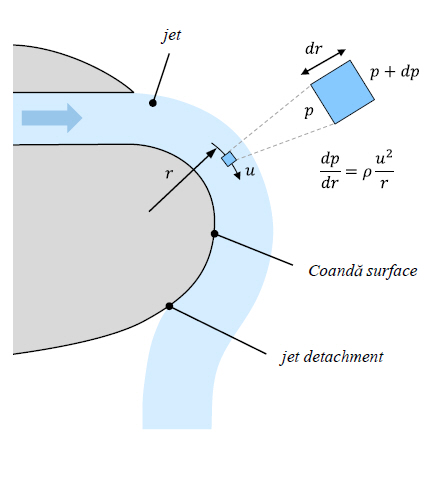
\includegraphics[width=0.45\textwidth]{coanda.jpg}
	\caption{Skizze zum Coand\^{a}-Effekt \cite{Stadlberger.2016}}
	\label{fig:coanda}
\end{figure}

Tritt ein Freistrahl in ein ruhendes Fluid ein, rei\ss{}t er an dessen R"andern das umgebende Medium mit. Um die Kontinuit"atsbedingung zu erf"ullen, entsteht am Au\ss{}enraum des Strahls eine Str"omung zur Strahlmitte, was als Entrainment-Effekt bezeichnet wird. In der N"ahe einer K"orperkontur wird das Nachstr"omen des Mediums unterbunden. In der Folge entsteht an der Wand ein lokaler Unterdruck und somit ein Druckgradient $dp$ quer zur Str"omungsrichtung. Dies f"uhrt zu einer Umlenkung des Freistahls in Richtung der Wand, wie in \abb{fig:coanda} ersichtlich ist. In der Folge entsteht ein Wandstrahl, welcher sich an die K"orperkontur anschmiegt \cite{Fernholz.1966}. 

Die Kr"ummung pr"agt dem Strahl eine Zentrifugalkraft auf, welche im Gleichgewicht mit der Resultierenden infolge des Druckgradienten $dp$ steht. Eine Erh"ohung der Wandkr"ummung ruft jedoch eine st"arkere Zentrifugalkraft hervor. Deshalb kann der Wandstrahl starken Kr"ummungen durch kleine Wandradien nicht folgen und l"ost ebenfalls ab \cite{Riedel.1971}.\\

Da es sich bei der Coand\^{a}-Str"omung um einen Wandstrahl handelt, existiert zur Grenzschicht eine zus"atzliche Reibungsschicht zum umgebenden Medium. Somit bildet sich ein Geschwindigkeitsprofil wie in \abb{fig:Wandstrahl} aus.


%nach unten gerückt

%\begin{figure}[h]
%	\centering
%	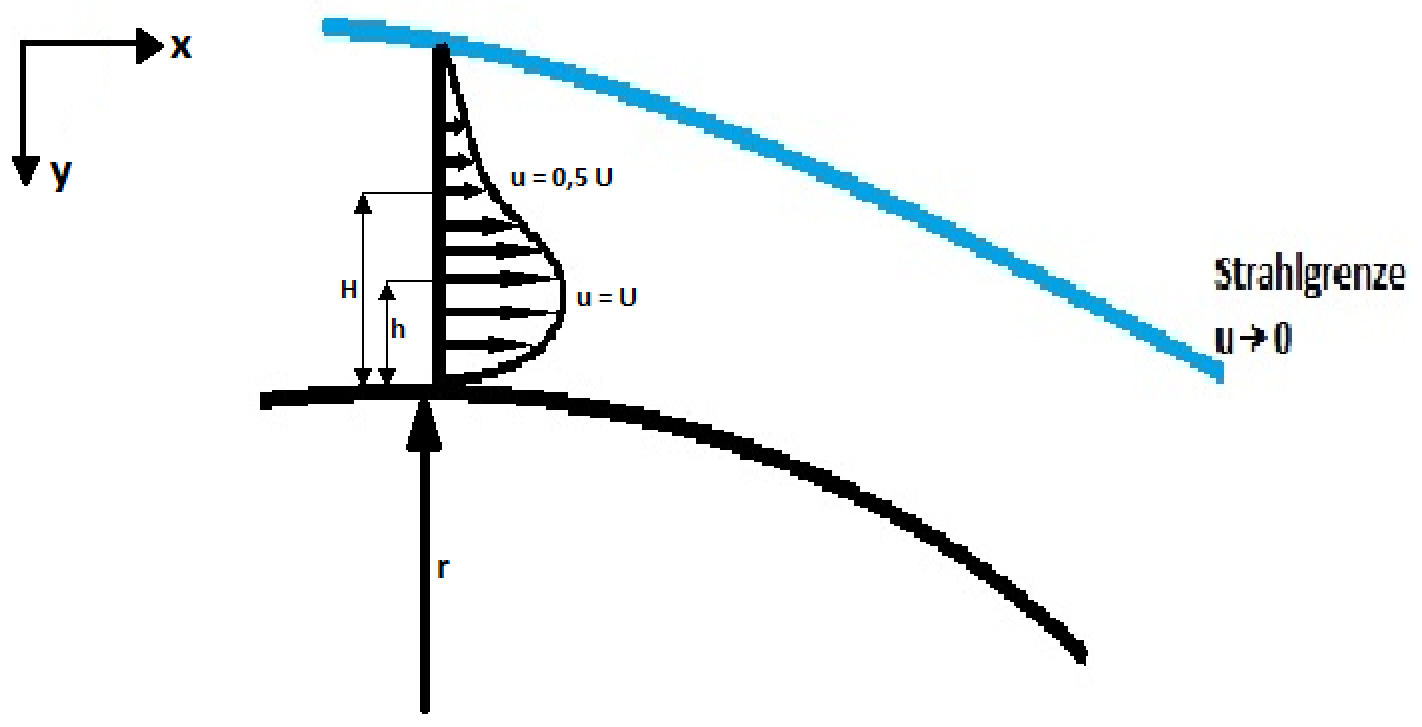
\includegraphics[width=0.7\textwidth]{Wandstrahl.jpg}
%	\caption{Geschwindigkeitsprofils eines Wandstrahls an einer konvexen K"orperkontur nach Riedel \cite{Riedel.1973}}
%	\label{fig:Wandstrahl}
%\end{figure}

Im zeitlichen Mittel ist die resultierende Zentrifugalkraft proportional zu $\frac{u^2}{r+y}$. Dabei ist die wirkende Zentrifugalkraft in der N"ahe des Maximums des Geschwindigkeitsprofils des Wandstrahls proportional zu $\frac{U^2}{r+\frac{H}{4}}$. Dabei ist $H$ die H"ohe des Strahls, was in unserer Konfiguration der Spalth"ohe entspricht. Die Zentrifugalkraft ist somit in der Strahlmitte aufgrund der h"oheren Geschwindigkeit gr"o\ss{}er als die auf Teilchen in der N"ahe der Strahloberfl"ache und in der N"ahe der K"orperkontur.


An der K"orperkontur ist die resultierende Zentrifugalkraft proportional zu $\frac{u^2}{r}$, an der Strahloberfl"ache jedoch nur zu $\frac{0,25 \cdot U^2}{r + H}$. Aus diesem Grund besteht die Tendenz von Teilchen in der N"ahe der Maximalgeschwindigkeit, zum "au\ss{}eren Rand und somit in das Gebiet der Strahlvermischung mit dem Umgebungsmedium abzudriften. Durch ihre geringere Zentrifugalkraft blockieren die Teilchen innerhalb des "au\ss{}eren Randes jedoch die nach au\ss{}en dringenden Teilchen und somit eine nach au\ss{}en gerichtete Bewegung. Infolgedessen treffen zus"atzliche Teilchen am Rand aufeinander, was eine Strahlvermischung bef"ordert.

Ein entgegengesetztes Verhalten findet sich in der N"ahe der K"orperkontur. Den Teilchen in Wandn"ahe wird eine kleinere Zentrifugalkraft als im Strahlzentrum aufgepr"agt. Weniger Kollisionen und somit eine geringere gegenseitige Beeinflussung benachbarter Teilchen sind die Folge. Dies reduziert den Turbulenzgrad verglichen mit einer ebenen Strahlstr"omung.
Stromabw"arts weitet sich die Mischbewegung vom Strahlrand zum Strahlkern und zur konturnahen Str"omung aus, weshalb der Turbulenzgrad infolge der Strahlvermischung steigt \cite{Riedel.1973}.\\

Wie bereits oben erw"ahnt wurde, wird am freien Rand das umgebende Fluid mitgerissen, was gleichzeitig zu einer Reduktion der kinetischen Energie des Strahls f"uhrt. Die daraus resultierende Verlangsamung der Coand\^{a}-Str"omung sorgt daf"ur, dass die Abl"oseneigung des Strahls mit der Laufl"ange zunimmt \cite{Fischer.2011}. Aus dieser Beobachtung heraus wurde der Anlegewinkel f"ur Coand\^{a}-Str"omung an einem Zylinder durch Newman definiert \cite{Newman.1961}. Dieser beschreibt das Verh"altnis vom Radius $R$ der konvexen K"orperkontur zur Ausdehnung $H$ des Strahls. Die Ausdehnung $H$ des Strahls wird durch die Spalth"ohe bestimmt, weshalb der Anlegewinkel eine fundamentale Beziehung geometrisch signifikanter Gr"o\ss{}en der Coand\^{a}-Fl"achen-Ausblasung beschreibt. Infolge h"oherer Zentrifugalkr"afte bei gro\ss{}en Wandkr"ummungen nimmt der Anlegewinkel bei kleinen $\frac{H}{R}$ und konstanten Ausblasimpuls zu. Wird die Spalth"ohe kleiner, erh"oht sich gem"a\ss{} der Kontinuit"atsgleichung die Ausblasgeschwindigkeit. Diese Geschwindigkeiterh"ohung sorgt f"ur eine Steigerung des Entrainment-Effektes und in Folge dessen ebenfalls des Coand\^{a}-Effektes \cite{Fischer.2011}.


\begin{figure}[h]
	\centering
	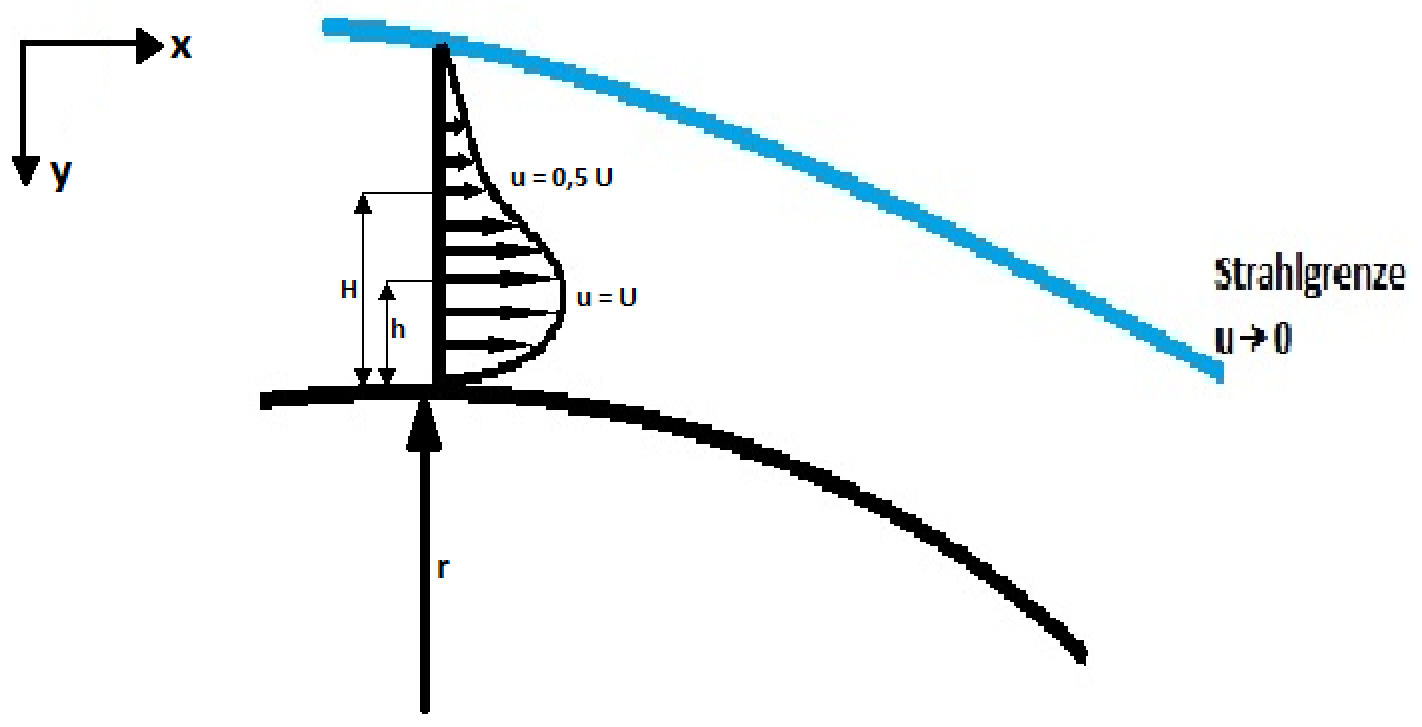
\includegraphics[width=0.7\textwidth]{Wandstrahl.jpg}
	\caption{Geschwindigkeitsprofils eines Wandstrahls an einer konvexen K"orperkontur nach Riedel \cite{Riedel.1973}}
	\label{fig:Wandstrahl}
\end{figure}

%%
%Da es sich bei der Coand\^{a}-Str"omung um einen Wandstrahl handelt, gibt es zur Grenzschicht eine zus"atzliche Reibungsschicht zum umgebenden Medium. Dies wird in \abb{fig:coanda} gezeigt. Da das Umgebungsmedium ruht, gibt es gem"a\ss{} Bernoulli keinen Druckanstieg entlang der konvexen Rundung, die Grenzschicht bleibt stabil. Aus diesem Grund haftet die Coand\^{a}-Str"omung l"anger an K"orperkontur an.






%%%%%%%%%%%%%%%%%%%%%%%%%%%%%%%%NORAS REICH ;) %%%%%%%%%%%%%%%%%%%%%%%%%%%%%%%%%%%%%%%%%%%%%%%%%
\newpage
\section{Aktive Str\"omungsbeeinflussung (NB)}

Stumpfe K"orper haben meist ein stufenartiges Ende, aus dem sich str"omungsmechanische Nachteile ergeben. Diese Nachteile sollen durch eine Anpassung der Geometrie des K"orpers oder durch die strukturelle Ver"anderung des Totwassers ausgeglichen werden.  Ziel ist es, den Basisdruck anzuheben und dar"uber den Druckwiderstand des K"orpers zu verringern \cite{Hucho.2011}.\\
%hier evtl ein paar passive verfahren
Die nachfolgende Arbeit konzentriert sich auf ein aktives Verfahren der Str"omungsbeeinflussung, weshalb im Folgenden einige bis jetzt realisierte Verfahren vorgestellt werden.

%-------------------------------------------------------------------------------------
Bearman \cite{Hucho.2011} hat als einer der Ersten die aktive Str"omungsbeeinflussung nachgewiesen. \abb{fig:Bearman} zeigt das verwendete Stumpfk"orpermodell. Dabei ist als Besonderheit auf die por"ose Basis \(A_{0}\) hinzuweisen, durch die zus"atzlich Luft am Ende des K"orpers ausgesto\ss{}en wird. Es werden zwei Ausblasequerschnitte \(A_{0}\) gew"ahlt, zum einen "uber einen Gro\ss{}teil der Fl"ache A und zum anderen "uber die H"alfte der Fl"ache zentriert in der Mitte angeordnet.
\begin{figure}[h]
	\centering
	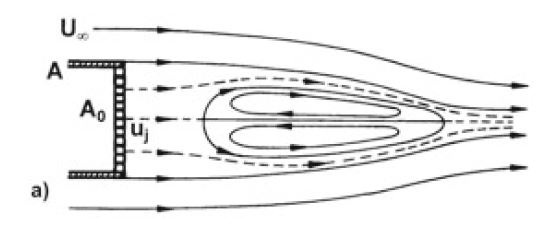
\includegraphics[width=0.5\textwidth]{KorperBearman.jpg}
	\caption{Stumpfk"orper mit Ausblasung von Bearman \cite{Hucho.2011}}
	\label{fig:Bearman}
\end{figure}\\
Aus seinen Experimenten \cite{Hucho.2011} hat sich ergeben, dass der Druck hinter dem K"orper mit wachsendem Volumenstrom zunimmt. Die austretende Luft sorgt daf"ur, dass die Str"omungsabl"osung vom K"orperende weggeschoben wird. Sie fungiert wie eine Trennplatte im Bereich der passiven Str"omungsbeeinflussung. Durch die erst weiter hinten stattfindende Verwirbelung, f"allt der Widerstand des K"orpers ab.

%-------------------------------------------------------------------------------------
Geropp und Odenthal beschreiben in \cite{Geropp.2000} Experimente zur Einblasung am Ende eines Kraftfahrzeuges "uber zwei Schlitze mit Nutzung des Coand\^{a}-Effekts (\abb{fig:Geropp}).
\begin{figure}[h]
	\centering
	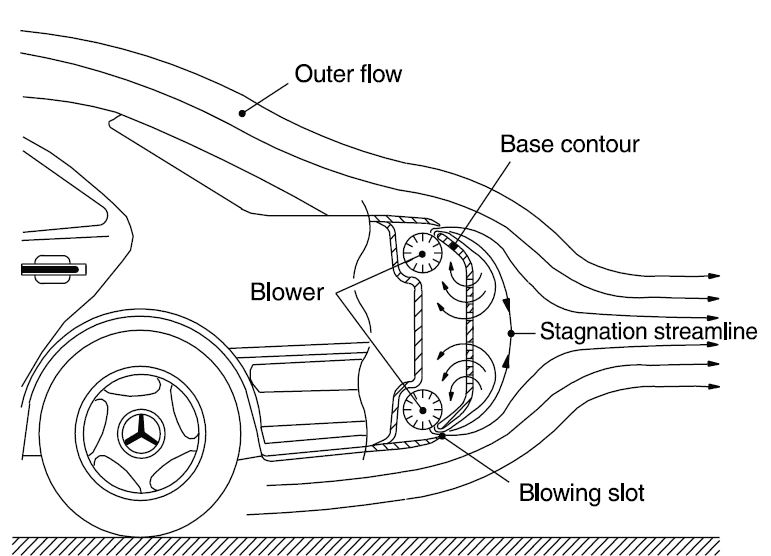
\includegraphics[width=0.5\textwidth]{KorperGeropp.jpg}
	\caption{Stumpfk"orper mit Ausblasung von Geropp \cite{Geropp.2000}}
	\label{fig:Geropp}
\end{figure}

Hierbei ist f"ur die Beeinflussung der Grenzschicht die Ausblasung bei hohen Geschwindigkeiten erforderlich. Durch den Coand\^{a}-Effekt wird die eingeblasene Luft in das Totwasser umgelenkt, wo sie wieder abgesaugt wird. Dadurch wird der Druck hinter dem Fahrzeug erh"oht und der Gesamtwiderstand verringert. Die Experimente zeigen, dass eine Druckerh"ohung von~50\% und eine Widerstandsverringerung um 10\% m"oglich ist. Au\ss{}erdem wird ein Energievorteil f"ur moderate Ausblasgeschwindigkeiten mathematisch festgestellt.

%--------------------------------------------------------------------------------------
In \cite{Barros.2016} wird zus"atzlich zu den vorher beschriebenen Verfahren die Ausblasung gepulst durchgef"uhrt. Dabei soll der Einfluss von Frequenz und Amplitude auf das Widerstandsverhalten untersucht werden.\\
In \abb{fig:Barros} ist der schematische Aufbau der gepulsten Ausblasung dargestellt. Diese wird "uber Ventile realisiert, die eine Rechteckkurve mit einem duty cycle von 40\% erzeugen. Der duty cycle gibt den prozentualen Anteil des ge"offneten Signalteils bezogen auf die gesamtm"ogliche "Offnung an. Direkt unter der Ausblastelle wird zus"atzlich eine Coand\^{a}-Fl"ache angebracht.\\
\begin{figure}[h]
	\centering
	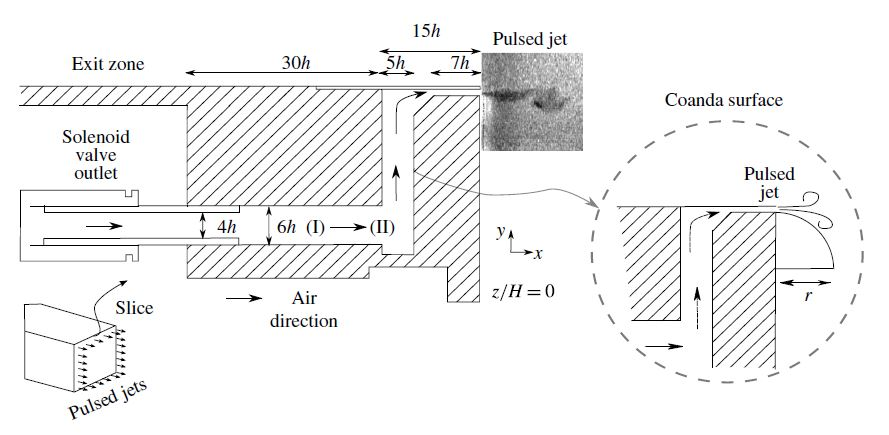
\includegraphics[width=0.7\textwidth]{KorperBarros.jpg}
	\caption{Gepulste Ausblasung von \cite{Barros.2016}}
	\label{fig:Barros}
\end{figure}

Mit steigender Frequenz und steigender Amplitude, wurde eine Umlenkung der Grenzschicht beobachtet. "Uber eine gepulste Einblasung, nahe der nat"urlichen Abl"osefrequenz der Str"omung, kann nach \cite{Barros.2016} der Widerstand am meisten (10\%) gesenkt werden. Bei zus"atzlicher Nutzung der Coand\^{a}-Fl"ache kann eine Reduktion von 20\% erreicht werden.

%-------------------------------------------------------------------------------------
Modi et al. \cite{MODI.1991} versuchen durch drehende Zylinder den Widerstand zu reduzieren. Dabei werden unterschiedliche Modelle genutzt. F"ur erste Versuche wird das Modell in \abb{fig:Modi3} und sp"ater der LKW (Truck) aus \abb{fig:Modi} verwendet.
\begin{figure}[h]
	\centering
	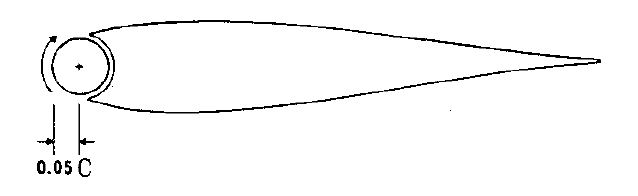
\includegraphics[width=0.6\textwidth]{KoerperModi3.jpg}
	\caption{Stumpfk"orpermodell mit Walze von Modi et al. \cite{MODI.1991}}
	\label{fig:Modi3}
\end{figure}

F"ur den K"orper in \abb{fig:Modi3} sind Str"omungsbilder (\abb{fig:ModiStr}) aufgenommen worden. Diese sind mit einem Anstellwinkel des K"orpers von 20 Grad entstanden. Das Verh"altnis der Drehgeschwindigkeit der Zylinder \(U_c\) bzgl. der Anstr"omgeschwindigkeit \(U\) wurde variiert.\\
\begin{figure}[h]
	\centering
	\begin{subfigure}[c]{0.4\textwidth}		
		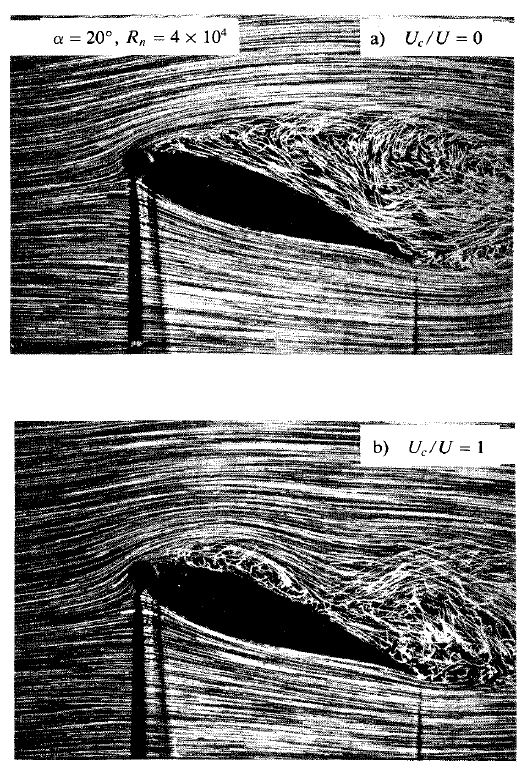
\includegraphics[width=0.7\textwidth]{ModiStr1.jpg}
	\end{subfigure}
	\begin{subfigure}[c]{0.4\textwidth}
		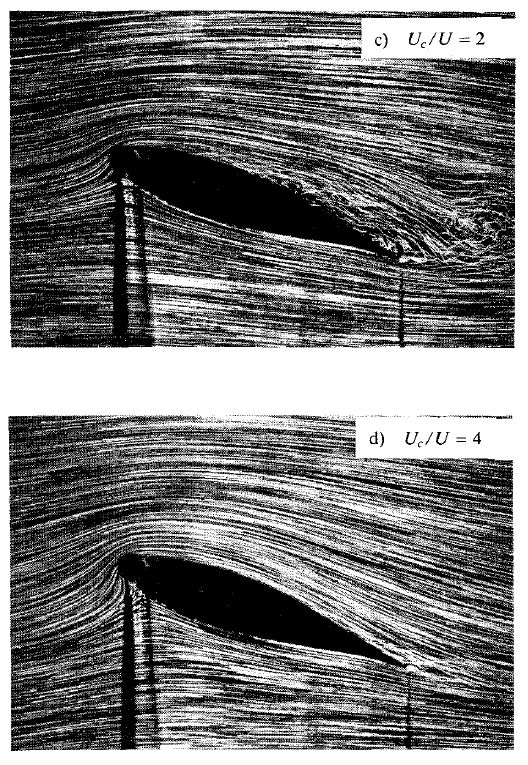
\includegraphics[width=0.7\textwidth]{ModiStr2.jpg}
	\end{subfigure}
	\caption{Str"omungsbilder von Modi et al. \cite{MODI.1991}}
	\label{fig:ModiStr}
\end{figure}

Auf den Str"omungsbildern (\abb{fig:ModiStr}) kann gut gesehen werden, dass bei nicht rotierenden Zylindern \(U_c/U=0\) (oben links) die Abl"osung stark ist im Vergleich zu \(U_c/U=4\) (unten rechts), hier drehen die Zylinder viermal schneller als die Anstr"omung.\\
\begin{figure}[h]
	\centering
	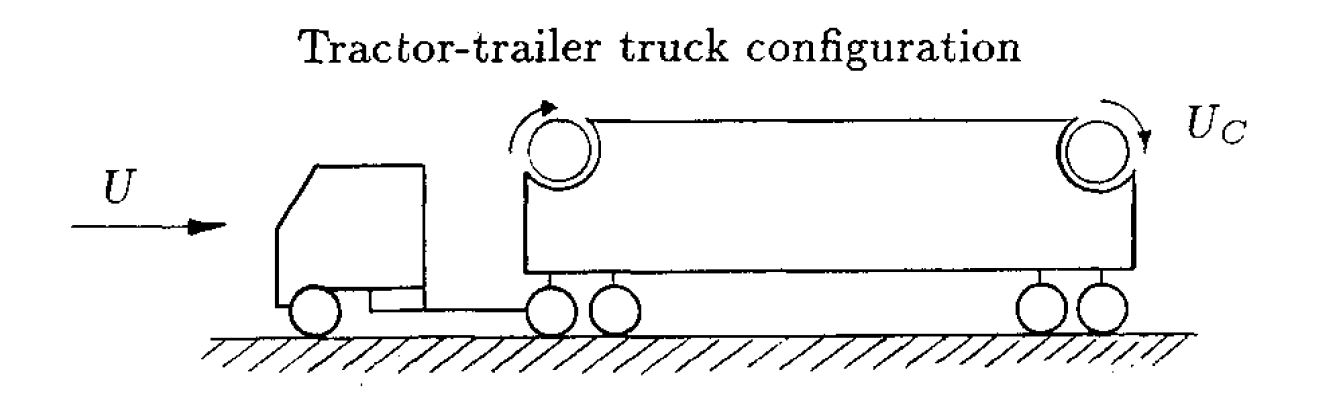
\includegraphics[width=0.6\textwidth]{KorperModi.jpg}
	\caption{Erstes Truckmodell von Modi et al. \cite{MODI.1991}}
	\label{fig:Modi}
\end{figure}
Bei den Versuchen am Truckmodell sind die Zylinder in einem ersten Veruch angeordnet, wie in \abb{fig:Modi} dargestellt. Dabei werden die Rauhigkeiten der Zylinder variiert. Es gibt einen glatten Zylinder, einen mit einer Rauhigkeit von 40 und einen mit 80. Au\ss{}erdem wird wieder das Verh"altnis der Drehgeschwindigkeiten der Zylinder \(U_c\) bzgl. der Anstr"omgeschwindigkeit \(U\) f"ur alle drei F"alle variiert. Daraus ergeben sich die Widerstandsreduktionen in \tab{tab:Modi}.\\
\begin{table}[h]
	\centering
	\begin{tabular}{lrr}
		\toprule
		Zylinder & Widerstandsreduktion [\%] & \(U_c/U\)\\
		\midrule
		glatt & 5 & 2\\
		Rauhigkeit 80 & 10 & 2.1\\
		Rauhigkeit 40 & 13 & 2.1\\
		\bottomrule
	\end{tabular}
	\caption{Widerstandsreduktion bei Modi}
	\label{tab:Modi}
\end{table}
Da der hintere Zylinder keinen Impuls in die Grenzschicht einbringen kann, wurde ein zweites Experiment mit anderer Konfiguration durchgef"uhrt. Dabei wurde ein Zylinder mit spiralf"ormiger Rille in der Oberfl"ache und einer mit einer Vielkeil-Verzahnung, deren Rillen parallel zur Drehachse verlaufen, verwendet. Die Position des ersten Zylinders bleibt unver"andert, der Zweite wird ans Ende des ersten Drittels der Truckoberseite positioniert (siehe \abb{fig:Modi2}).\\
\begin{figure}[h]
	\centering
	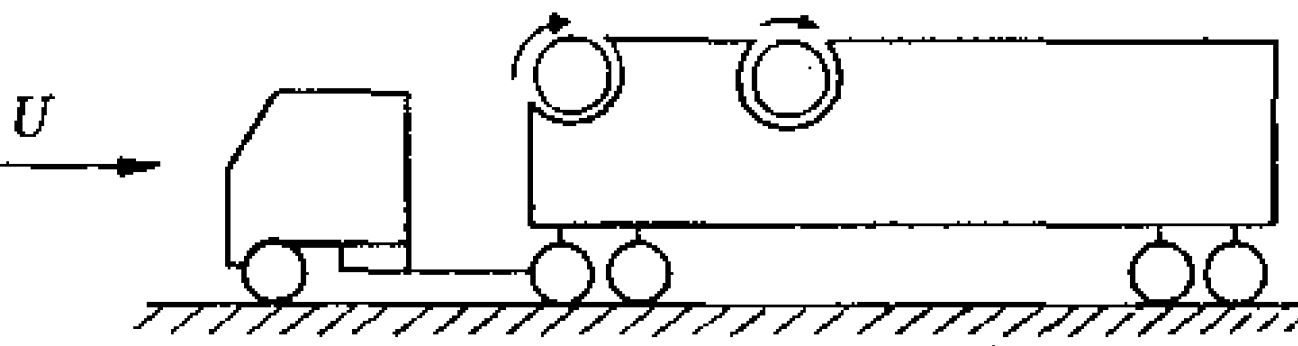
\includegraphics[width=0.5\textwidth]{KoerperModi2.jpg}
	\caption{Zweites Truckmodell von Modi et al. \cite{MODI.1991}}
	\label{fig:Modi2}
\end{figure}\\
Der spiralf"ormige Zylinder erzielte das gleiche Ergebnis, wie der Zylinder mit einer Rauhigkeit von~40 im ersten Experiment. Der Vielkeil-Verzahnungszylinder hat allerdings einen gro\ss{}en Einfluss auf den Widerstand. Bei alleiniger Betrachtung des vorderen Zylinders wird eine Reduktion von~29\% erreicht, beide Zylinder erreichen bis zu 41\%.

%------------------------------------------------------------------------------------
In \cite{Gong.2015} werden eine r"uckwertsgewandte Stufe, ein 2D-Modell und anschlie\ss{}end ein 3D-Model (\abb{fig:Gong}) untersucht. Das besondere dabei ist die Anregungsform "uber einen Lautsprecher, der ein monofrequentes, sinusf"ormiges Anregungssignal durch kleine L"ocher in die Str"omung gibt. Durch die Sinusfunktion wird erreicht, dass die eingestr"omte Masse "uber eine Periode betrachtet gleich Null ist. Neben der Untersuchung im Windkanal wurde eine instation"are Simulation entwickelt und validiert, welche einen genauen Einblick in die Wirbelstrukturen erm"oglicht.
\begin{figure}[h]
	\centering
	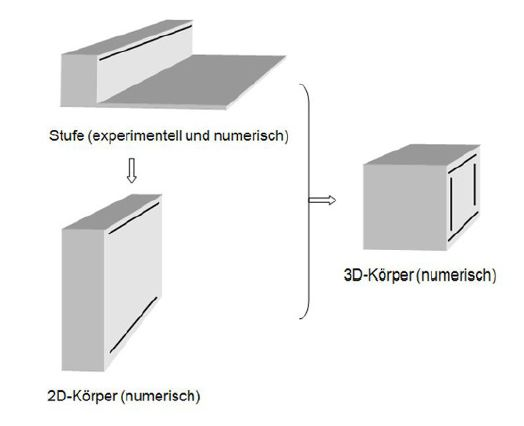
\includegraphics[width=0.5\textwidth]{KoerperGong.jpg}
	\caption{Modelle nach Gong \cite{Gong.2015}}
	\label{fig:Gong}
\end{figure}\\
Bei einer hochfrequenten Anregung kann die Bildung von Wirbeln unterdr"uckt werden. Dadurch wird der Druck hinter der Basis erh"oht und der Luftwiderstand des K"orpers sinkt.

%------------------------------------------------------------------------------------
Alle bisher vorgestellten Verfahren haben nur eine Steuerung des Vorgangs betrachtet. Darauf aufbauend wird in \cite{Henning.2008} zus"atzlich eine Regelung des Mechanismuses der Str"omungsbeeinflussung eingef"uhrt. Dabei sollen "au\ss{}ere St"orungen ber"ucksichtigt werden, wie beispielsweise sich gegenseitig beeinflussende Kraftfahrzeuge.\\
Im Rahmen der Arbeit \cite{Henning.2008} wurden unterschiedliche K"orper "ahnlich zu denen in \abb{fig:Gong} analysiert.
%\begin{figure}[h]
%	\centering
%	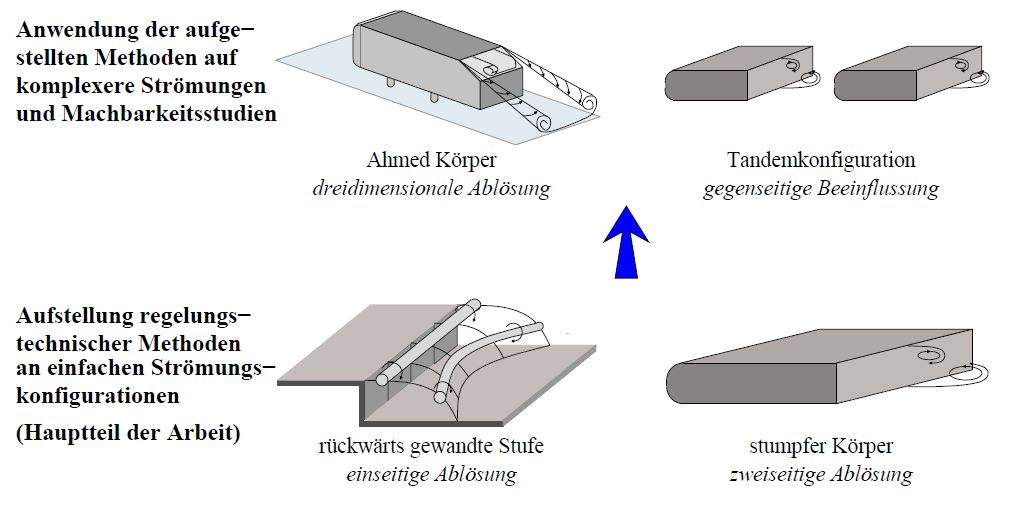
\includegraphics[width=0.8\textwidth]{KorperHenning.jpg}
%	\caption{betrachtete Modelle f"ur Auslegung der Regelung \cite{Henning.2008}}
%	\label{fig:Henning}
%\end{figure}\\
An der r"uckw"arts gewandten Stufe wurde erfolgreich die Wiederanlegel"ange "uber einen segmentierten Schlitz an der Stufenkante geregelt. Au\ss{}erdem konnte eine Unterdr"uckung von St"orungen erreicht werden. Das Ganze wurde "uber eine Robuste Regelung realisiert.\\
Am stumpfen K"orper wurde mit Hilfe einer Phasenregelung an Ober- und Unterseite eine Widerstandsreduzierung von bis zu 15\% erreicht.\\
Die Tandemkonfiguration (zwei K"orper hintereinander) wurde im Rahmen einer Machbarkeitsstudie \cite{Henning.2008} untersucht und f"ur zuk"unftige Arbeiten als sinnvoll betrachtet. Dabei geht es um die St"oreinfl"usse, die der erste K"orper auf den Zweiten hat und wie dieser die St"orung "uber eine Regelung beseitigen kann, sodass auch beim zweiten K"orper eine Widerstandsreduzierung m"oglich ist.\\
Die Regelung stellt einen weiteren Schritt in Bezug auf eine Widerstandsreduktion von Stumpfk"orpern dar. Im Rahmen dieser Arbeit wird eine Regelung nicht mit betrachtet, da erst das neue Konzept untersucht werden muss.
